\section{Diagnostics techniques} \label{section:diagnostics-techniques}
Fault identification in the rotating machinery is one-class or multi-class classification problem acting in a semi-supervised manner because labels for degraded conditions are scarce in practice. The automation goals in monitoring can be broadly categorized as anomaly detection and recognizing the momentary fault type.

The guiding principles for algorithm selection are simplicity in terms of their straightforward visual explanation for the production managers, and the ability to progressively improve the model on the streaming data to address peculiarities in individual machine constructions.

\subsection{Novelty detection}
Anomaly, novelty, or outlier detection determines whether a health status deviates considerably from the baseline profile. The expert can then step in and diagnose the machine after the notice. Anomaly is a rare observation different from the others raising suspicion that it was created with an unrelated behavior~\cite{aggarwal_outlier_2016}. The observations get assigned anomaly scores, and those over the threshold are novelties.

The measurements coming in the steaming fashion have to be processed in a single pass. The detection model must deal with the minimal admissible assumptions about the nature of the input events. The outliers are based on non-parametric statistical models, nearest-neighbor clustering, and isolation-based approaches~\cite{gervasi_anomaly_2020}.
\bigbreak

\textbf{DenStream} is a density-based algorithm adapted from DBSCAN to cluster streaming data of arbitrarily shaped groups. Samples it includes in the first step into coherent clusters are core data points in each other's neighborhoods. Core points have at least \emph{MinPts} ($\mu$) points in their neighborhood of radius \emph{Eps} ($\varepsilon$) units. Then non-core points in the proximity area of the core point are attached to the cluster containing it~\cite{aggarwal_data_2014}.

\begin{figure}[ht]
    \centering
    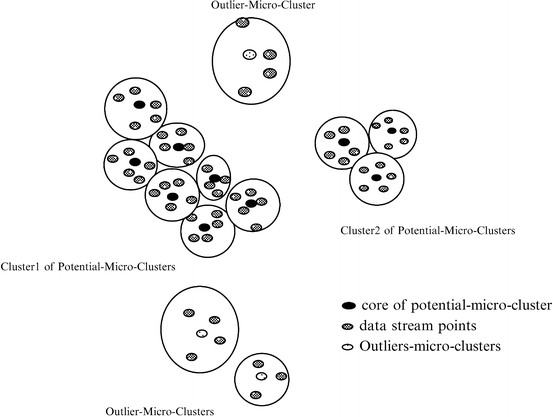
\includegraphics[width=0.8\textwidth]{assets/DenStream.png}
    \caption{DenStream~\cite{amini_density_2012}}
    \label{fig:denstream}
\end{figure}

In the online maintenance phase, DenStream summarizes the nearby observations into core \emph{micro-clusters} that can be potential or outlier \emph{micro-clusters} (Fig.~\ref{fig:denstream})~\cite{ghesmoune_state---art_2016}. The (outlier) \emph{o-micro-clusters} can grow into (potential) \emph{p-micro-clusters} when they encompass $\beta \mu$ points. The outliers are discounted after some time in accordance to the decay function: $f(t) = 2^{-\lambda t}$ or below lower weight limit $\xi$. The on-demand offline stage runs DBSCAN over the approximate representation in micro-clusters to deliver final apportionment~\cite{cao_density-based_2006}.
\bigbreak

\textbf{Half-Space Tree} (HS-Tree) stands upon the concept of Isolation forest. It assumes that random splitting of each axis in the feature space will isolate outliers to their separate divisions sooner than non-deviant observations~\cite{gervasi_anomaly_2020,torres_automatic_2022}. This ensemble of trees is better suited for batch setting. HS-Tree stands out in adapting to changing streams because it is trained solely on normal data, requires constant memory, and is faster than density-based methods~\cite{tan_fast_2011}.

\begin{figure}[ht]
    \centering
    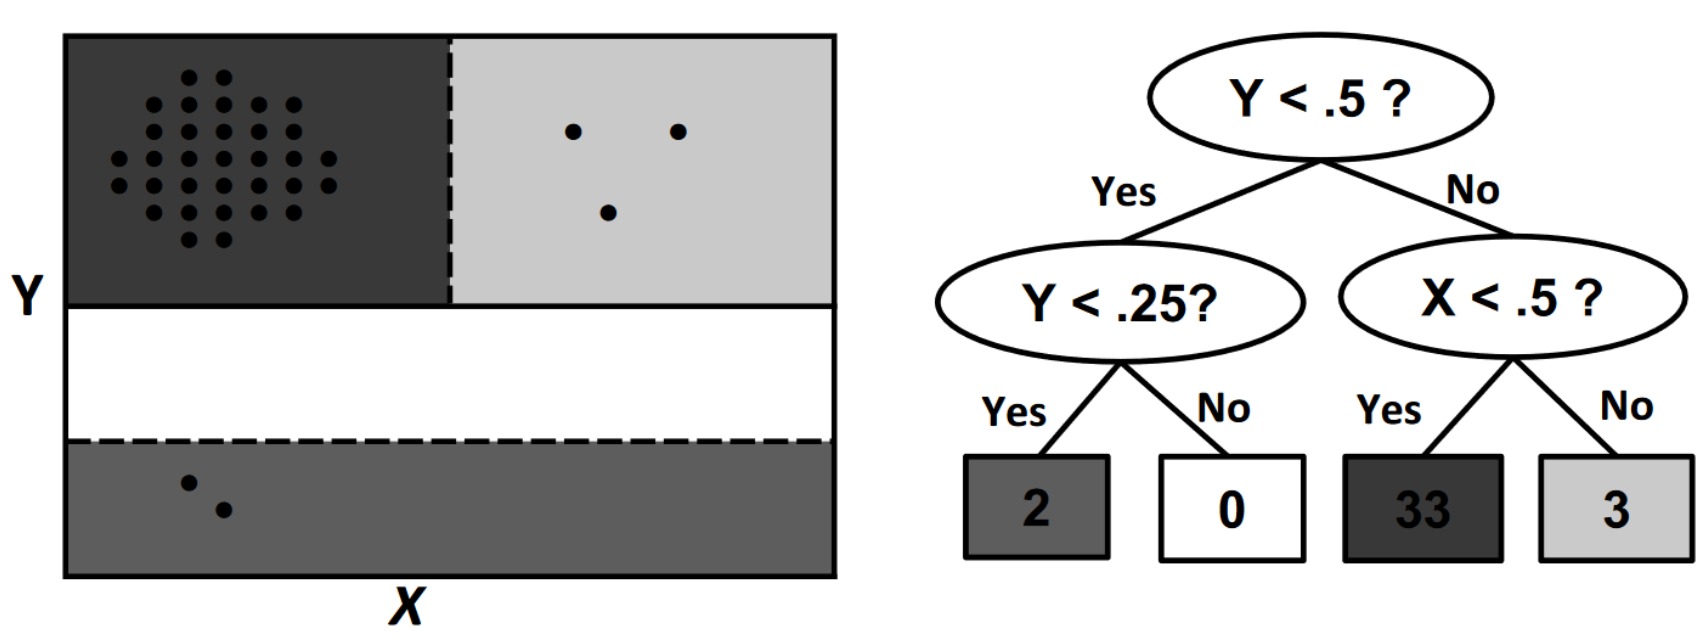
\includegraphics[width=0.8\textwidth]{assets/HS-Tree.png}
    \caption{Half-space tree~\cite{tan_fast_2011}}
\end{figure}

A full binary tree is built before the novelty detection begins by splitting tree nodes along the divisions in the randomly chosen perpendicular planes. The node stores its depth, value limits of the axis bisection (half-space), count of contained data points (mass) in two consecutive windows, and link to both child nodes~\cite{tan_fast_2011}. 

The anomaly profile in the latest window is always compared to the predecessor reference window. After the latest window is filled up it replaces the reference window. It suffices to use a window size of 250 and 25 tree ensemble~\cite{tan_fast_2011}.

\subsection{Classification}
Accurate multi-class classification of machine fault causes out of the characteristics of known ones is a much more difficult task than novelty detection. Universal enough fault baseline has to be recorded and transformed into feature space. Interactions among fault manifestations have to be accounted for. We are aware of rapid advances in knowledge transfer for deep neural networks~\cite{maurya_condition-based_2021}. So far, solutions seem not production ready. Therefore, we opt to use a more rudimentary model.
\bigbreak

\textbf{K-nearest neighbors} (kNN) assigns the data point to the class where the majority of $k$ closest instances belong (Fig.~\ref{fig:knn}). This means it can work in the semi-supervised environment because it can infer labels just from knowing a few annotations.

\begin{figure}[ht]
    \centering
    \begin{subfigure}[b]{0.49\textwidth}
        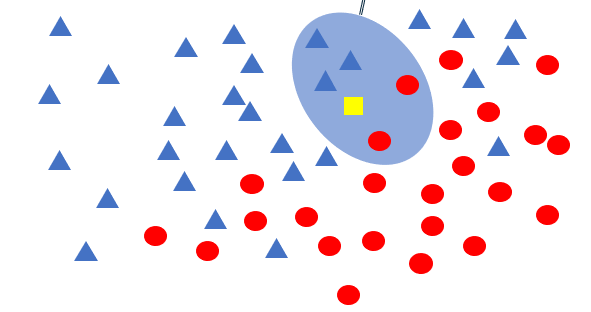
\includegraphics[width=\textwidth]{assets/kNN.png}
        \caption{kNN with k = 5}
        \label{fig:knn}
    \end{subfigure}
    \hfill
    \begin{subfigure}[b]{0.49\textwidth}
        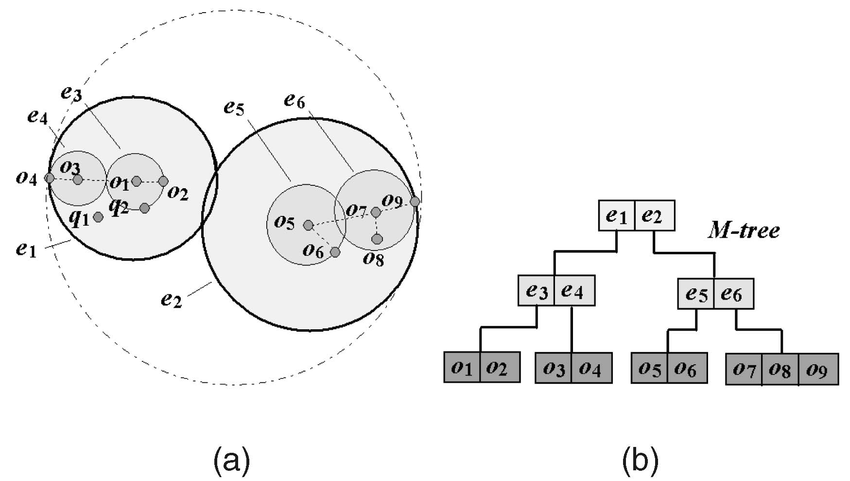
\includegraphics[width=\textwidth]{assets/M-tree.png}
        \caption{M-tree data structure}
        \label{fig:m-tree}
    \end{subfigure}
    \caption{Nearest neighbors classification algorithm~\cite{chen_skyline_2009}}
\end{figure}

The sense of distance between feature vectors $\mathbf{x}$, $\mathbf{y}$ have to be defined, so several metrics are available like \emph{Euclidian distance}, \emph{Mahalanobis distance}, or \emph{RBF kernel} (Tab.~\ref{tab:knn-distance})~\cite{sheng_review_2020}. The demanding neighborhood queries are sped up by a Metric search tree data structure such as \emph{M-Tree} (Fig.~\ref{fig:m-tree}). The optimal $k$ parameter is set in supervised learning according to the breaking point in the elbow curve that plots choices of $k$ against the error rate.

\begin{table}[ht]
\centering
\renewcommand{\arraystretch}{2}
\begin{tabular}{|l|l|}
\hline
\textbf{Distance}     & \textbf{$d(\mathbf{x}, \mathbf{y})$}                                   \\ \hline
Euclidian distance    & $ \sqrt{\sum_{i = 1}^{n}(x_i - y_i)^2} $                               \\ \hline
Mahalanobis distance  & $ (\mathbf{x} - \mathbf{y})^T C^{-1} (\mathbf{x} - \mathbf{y}) $       \\ \hline
Radial basis function & $ \exp\left(-\frac{\lVert \mathbf{x} - \mathbf{y} \rVert^2}{t}\right) $ \\ \hline
\end{tabular}
\caption{Distance metrics for kNN}
\label{tab:knn-distance}
\end{table}

Nearest-neighbour classifier has been successfully applied in machinery fault diagnostics. On the CWRU bearing dataset, the kNN with the accuracy of 96.2\% slightly outperformed SVM (95\%) on the combination of time and frequency-domain features, time-domain features - kNN 91.2\%, SVM 88.8\%, and frequency domain features - kNN (98.8\%), SVM (96.2\%)~\cite{jamil_feature-based_2021}. 

Comparison of kNN and KLDA on a feature set consisting of average, kurtosis, skewness, and standard deviation vectors in each domain has been conducted, achieving a data reduction rate of 95\%. Best accuracies were reached for PSD features with 99.13\% with KLDA and 96.64\% with KNN classifiers and Mahalanobis metric. The sampling frequency was set at 40 kHz~\cite{altaf_new_2022}. Despite kNN lagging in accuracy, we have to keep in mind annotations for faults were complete and machine learning was not tested in a streaming context.
